\chapter{Estado del arte}

Aquí se encontrará la parte teórica del proyecto. Se desglosará en que consiste la identificación de tráfico y 
las distintas técnicas que existen. También se hablará de Bro \cite{broindex}, el NMS que se usará para 
llevar a cabo el desarrollo del módulo. Se introducirá en que consiste, cómo gestiona los eventos y sus 
funcionalidades, así como la posibilidad de ampliar estas.

\intro Por último se presentará de forma teórica en que consiste el emparejamiento de flujos y de qué forma 
se podría usar para identificar el tráfico.

\section{Identificación de tráfico}

La identificación de tráfico, por si sola, no clasifica el tráfico. Solamente proporciona información obtenida 
de los paquetes, pudiendo ser los paquetes ordenados por distintas características una vez que ha 
sido identificado, por ejemplo la clase a la que pertenece.

\intro Por lo tanto la identificación del tráfico de la red es esencial para realizar una clasificación 
posterior, la cual se podrá analizar en busca de amenazas o intrusos. Para poder identificar el tráfico será 
necesario realizar algún método que sea práctico y eficiente.

\subsection{Técnicas de identificación de tráfico}

Existen varias técnicas de identificación de tráfico, como ya se explicó anteriormente. Estas técnicas son 
el paso previo a la clasificación del tráfico. Podría considerarse que son el paso intermedio a la clasificación. 
El tráfico, hasta ahora, se puede identificar de la siguiente forma.

\begin{itemize}
\item Por los puertos de la capa de transporte, establecido por IANA. \cite{iana}
\item Por el contenido del paquete o DPI. \cite{payload}
\item Por la aplicación de técnicas de aprendizaje automático sobre estadísticas de tráfico, machine 
learning. \cite{learning}
\end{itemize}

\intro En los siguientes apartados se verán de una forma más detallada.

\subsection{Identificación de tráfico basada en flujos}

En este ámbito se encuentran dos de las tres técnicas. Se detallarán a continuación.
\begin{itemize}

\item Identificación basada en los puertos de la capa de transporte. \cite{iana}

\intro Esta técnica consiste en identificar el tráfico dependiendo de los puertos de la capa de transporte, 
fue diseñada por IANA \cite{ianaexplicacion}. 

\intro IANA es la organización que se encarga de asignar los protocolos 
de Internet, algunos nombres de dominios y coordinar la asignación de direcciones IP. 

\intro Entonces, IANA es quien asigna el número de puerto a los distintos protocolos, haciendo que se pueda 
identificar el tráfico por el número de puerto al que se envía. Este sistema tiene el inconveniente de que 
ahora mismo, se están desarrollando multitud de aplicaciones web, las cuales se conectan mediante el 
puerto 80, es decir, mediante el protocolo HTTP. Pero esto no es cierto, pues se puede hacer que cualquier 
aplicación envíe información por el puerto 80, sin que sea HTTP, lo cual daría como resultado una mala 
identificación y posterior clasificación.

\item Identificación basada en la aplicación de técnicas de aprendizaje automático sobre estadísticas 
de tráfico \cite{learning}, se aplica sobre flujos.

\intro Esta clasificación es muy sencilla. Consta de algoritmos de aprendizaje automático, los cuales se 
dedican a realizar análisis estadísticos. De esta forma aprenden las características determinadas de 
los flujos. Este tipo de clasificación tiene un porcentaje de acierto del 95\%, según se puede leer en el 
artículo \cite{comparacion}.
\end{itemize}

\subsection{DPI}

\begin{itemize}

\item Identificación basada en el contenido del paquete o DPI. \cite{payload}

\intro Esta técnica de identificación consiste en analizar los paquetes, más allá de su cabecera. 
La Inspección Profunda de Paquetes, DPI por sus siglas en inglés, \textit{Deep Packet Inspection}. 
Esta técnica lo que hace es analizar todos los paquetes en busca de cadenas que se repitan, además 
de las IP's y los puertos. Una vez que tiene una cadena, la usa para buscar paquetes que tienen ese patrón, 
de esta forma establece un patrón de identificación.

\intro Esta técnica es útil para buscar virus, intrusiones y demás. Suele ser usada por los proveedores de 
servicios de Internet, ISP, por sus siglas en inglés \textit{Internet Service Provider} y grandes empresas. 
Se puede decir que es una técnica que no respeta la privacidad, pues entra dentro de la información del paquete, 
más allá de la cabecera. Aunque en el caso de una gran empresa si puede hacerse, pues si se está en la red propia 
no es delito mirar la información que contienen los paquetes. 

\intro En algunos países, como Alemania, donde es ilegal el uso de \textit{torrents}, 
las autoridades pueden pedir información al proveedor de servicios sobre uno de sus clientes, si cree que este 
está infringiendo la red, por lo que esta técnica es ideal para este tipo de cometidos.

\intro Además de para lo descrito, esta técnica también es ideal para saber si se está 
siendo atacado. \cite{dpiaproximacion}
\end{itemize}

\section{BRO}

Bro \cite{broindex}, es un analizador de tráfico de red de código abierto. Al ser de código abierto permite 
ser usado por quien lo desee sin necesidad de pagar licencias. Funciona sobre sistemas basados en Linux y 
Mac OS X. Una de sus principales características es la posibilidad de buscar amenazas en la red que 
se esté monitorizando.

\begin{figure}[H]
  
\includegraphics[width=0.5\textwidth]{imagenes/logo-bro.png}
  \centering
  \caption{Logo de Bro.}
\end{figure}

\intro No tiene interfaz gráfica, por lo que su gestión se realiza desde la linea de comandos. Cuando se analiza 
tráfico, Bro generará unos registros, los cuales están divididos en función de parámetros definidos por Bro.

\intro Bro incorpora la posibilidad de introducir funcionalidades nuevas, mediante la programación en su 
propio lenguaje de \textit{scripting}, del mismo nombre. Esto se desarrollará más adelante y en la 
parte de implementación se podrá ver cómo se desarrolla y algunos ejemplos de código escrito en Bro.

\intro El lenguaje de scripting está orientado a trabajar con eventos. Por lo tanto para añadir una 
nueva funcionalidad a Bro habrá que usar los eventos que ya tiene Bro y crear la función a partir de ahí.

\intro Bro está estructurado de forma que todos los flujos de paquetes que analiza son procesados por el motor de eventos. Este motor convierte los flujos de paquetes en eventos, de forma que es más sencillo trabajar con ellos. 
Una vez que los eventos son procesados se generarán los registros correspondientes. \cite{broarquitectura}

\begin{figure}[H]
  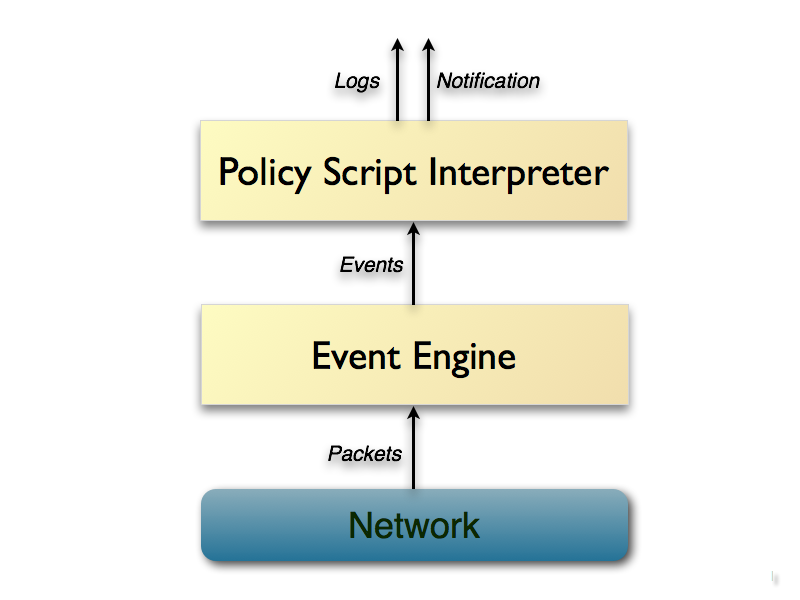
\includegraphics[width=0.5\textwidth]{imagenes/arquitectura-bro.png}
  \centering
  \caption{Arquitectura de Bro.}
\end{figure}

\subsection{Funcionalidades básicas de BRO}

La funcionalidad básica de Bro es el análisis del tráfico de la red, en la cual se esté ejecutando. 
Mientras que se encuentra ejecutándose, genera registros o \textit{logs} en texto plano que se 
podrán leer usando un editor de texto. Si se analiza un archivo \textit{pcap} los logs no cambiarán. Sin 
embargo si se analiza tráfico a tiempo real, los registros se irán actualizando a medida que pase el tiempo. 
Algunos \textit{logs} que se generan son los siguientes.

\begin{itemize}
\item \textit{dpd.log}. Consiste en un resumen de los protocolos encontrados en puertos que no son estándar.
\item \textit{dns.log}. Contendrá toda la actividad correspondiente al \textit{DNS}
\item \textit{ftp.log}. Un registro de la actividad a nivel de sesión de \textit{FTP}.
\item \textit{files.log}. Un resumen con los archivos transferidos a través de una red. Incluye 
protocolos \textit{HTTP, FTP y SMTP.}
\item \textit{http.log}. Registro de toda la actividad \textit{HTTP} con sus réplicas.
\item \textit{ssl.log}. Un registro de las sesiones \textit{SSL}, incluidos los certificados que se utilizan.
\item \textit{weird.log}. En este \textit{log} se guarda la información correspondiente a actividad 
inesperada o rara a nivel de protocolo. Al analizar gran cantidad de tráfico no es muy útil, pues ocurren 
muchas cosas raras, pero a pequeña escala es bastante interesante para detectar intrusiones y demás.
\item \textit{conn.log}. Aquí se puede ver la información correspondiente a conexiones  \textit{TCP, UDP e ICMP}.
\end{itemize}

\intro Para más información sobre \textit{logs} generados por una monitorización de Bro lea \cite{brologs}.

\intro Ahora con toda esta información, el administrador del sistema podrá determinar si existen amenazas en 
la red.

\subsection{Eventos y trazas}

La programación en Bro no es secuencial, no se escribe un \textit{script} y se espera que se ejecute en el orden 
en el que está escrito. Es programación orientada a eventos. Por lo tanto depende de cuando se den los eventos 
en el análisis ese será el orden.

\intro Un evento se da cuando Bro detecta un \textit{comportamiento}, por ejemplo cuando detecta un paquete 
de respuesta \textit{UDP}. Por lo tanto la programación deberá de estar pensada en función de los eventos 
disponibles.

\intro Dentro de cada evento se podrá hacer lo que se desee, con la información que capture ese evento. Si 
el evento captura información de una conexión \textit{TCP}, se tendrá que trabajar con esa información y las 
distintas variables globales que se hayan definido previamente.

\intro Una traza es una captura del tráfico de una red. Con casi cualquier programa de diagnóstico se puede 
realizar capturas de red. En la propia web de Bro se encuentran algunos archivos de trazas de red, en 
formato \textit{pcap}, de forma que se puedan realizar pruebas sobre ellos sin necesitar realizar una 
traza propia.

\intro En el caso de Bro se podrá generar trazas de red mediante un script de Python
\cite{brotrace}, el cual se puede descargar desde el repositorio de GitHub de Bro. Con dicho script también 
se podrá trabajar sobre la traza, separando el tráfico entrante del saliente, desglosando en distintos registros 
el tipo de tráfico y demás.


\subsection{Incorporación de funcionalidades}

La incorporación de funcionalidades a Bro es una de las características que más llaman la atención. Gracias 
a esto se podrá realizar un análisis muy personalizado usando un script creado por el administrador de redes. De 
esta forma podrá filtrar el tráfico de una determinada IP mientras se sigue analizando el tráfico de forma normal, 
con los registros que genera Bro de forma automática. Es una forma muy sencilla de comprobar si realmente alguien 
dentro de la red tiene un comportamiento extraño.

\intro A la hora de incorporar funcionalidades a Bro se puede hacer todo lo que se desee. Una búsqueda rápida 
por GitHub arrojará una gran cantidad de personas que aportan nuevos scripts a Bro \citep{gitbeacon}. Ahora lo 
ideal sería incorporar un módulo, de forma que si el resto de la comunidad lo desea pueda hacer uso de 
él, solamente llamando a las funciones que forman ese módulo.

\section{Emparejamiento de flujos}

La técnica de emparejamiento de flujos, fue planteada por el departamento de Teoría de la Señal, 
Telemática y Comunicaciones, \textit{TSTC}, de la Universidad de Granada, en el año 2011 \cite{presentacion}. 
Luego en el año 2013, el departamento realizó pruebas de la técnica de identificación en un entorno de 
laboratorio \cite{comparacion}.

\intro En el emparejamiento de flujos, la idea de la que se parte es muy sencilla. Si dos paquetes comparten 
IP's de origen y destino, y puertos de origen y destino, se podrá decir que esos dos paquetes pertenecen a 
la misma clase. Una vez que están identificados como pertenecientes a la misma clase, lo que se debe de hacer 
es comparar los tiempos de esos paquetes, de forma que sean coherentes en el flujo. Si son muy lejanos en el 
tiempo, se podrá descartar que pertenezcan al mismo flujo. Esta idea se puede ver en \cite{comparacion} de una 
forma mucho más técnica.

\intro En el mismo artículo se encuentra la fórmula que se sigue para el emparejamiento.

\begin{equation*}
	F(x,y)=
 	\begin{cases}
	  G(x,y), & NIP(x,y) \geq 1 \\
	  -\infty, & \text{en otro caso}
	 \end{cases}
\end{equation*}

\intro Donde tenemos que G(x,y) se corresponde con la siguiente función:

\begin{displaymath}
G(x,y) = |NIP(x,y) – 1| + 1 / (dp1(x,y) + k1) + 1 / (dp2(x,y) + k1) + 1 / (dt(x,y) + k2)
\end{displaymath}

\intro Las variables de la función son las siguientes: 

\begin{itemize}
\item \textit{x}: Primer paquete a comparar.
\item \textit{y}: Segundo paquete a comparar.
\item \textit{NIP(x,y)}: Es el número de paquetes analizados con las mismas características.
\item \textit{dp1(x,y)}: Se corresponde con los puertos de origen de los dos paquetes.
\item \textit{dp2(x,y)}: Serán los puertos de destino de los dos paquetes.
\item \textit{k1}: Es una variable definida previamente.
\item \textit{k2}: Es otra variable definida antes del comienzo del análisis. En trabajos anteriores esta variable 
y la anterior suelen estar definidas entre 1 y 10000.
\item \textit{dt}: Es la diferencia de tiempo existente entre los tiempos de inicio de los 
paquetes o \textit{timestamps}.
\end{itemize}

\intro Con esta fórmula se obtendrá un número, el cual será comparado con un umbral que se define previamente. Si 
el umbral definido es pequeño tendremos más flujos emparejados. Si el umbral es mayor serán menos los flujos 
que serán emparejados, al no cumplir los requisitos.

\intro El emparejamiento de flujos, por si mismo, sólo identifica el tráfico, por lo tanto se 
necesitará otra técnica para clasificar el tráfico.
